\section{Fundamentals of Interfacing}
\subsection{Basic Interface Structure \embsys{249}{6.1}}
\vspace{-0.5cm}
\begin{minipage}{9cm}
	\begin{itemize}
		\item Power Source
		\item Clock Oscillators
		\item Power on Reset
		\item Booting Function
	\end{itemize}
\end{minipage}
\begin{minipage}{5cm}
	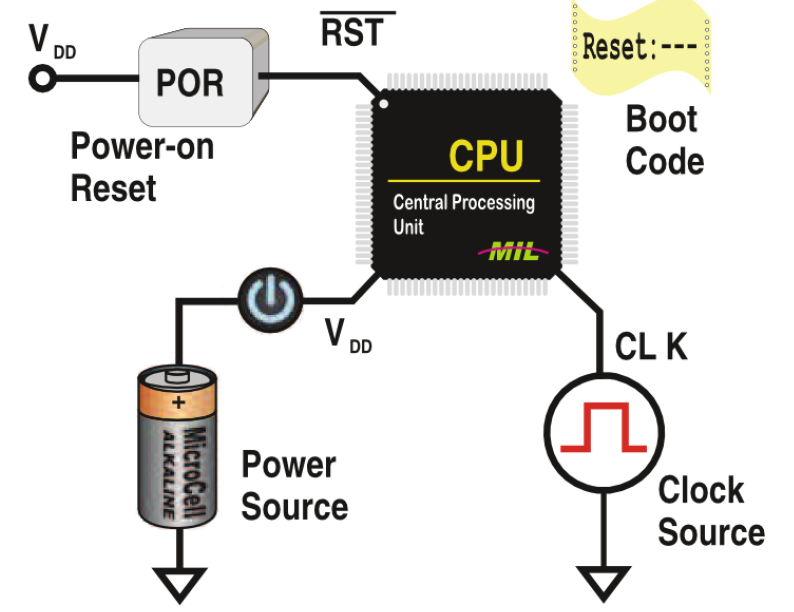
\includegraphics[width=6cm]{images/power.png}
\end{minipage}

\subsection{Power Sources \embsys{250}{6.2}}
\begin{minipage}{13cm}
\begin{itemize}
	\item Provide Power to CPU and its peripherals
	\item Require Steady Voltage
	\item Establish reference Levels for internal Operations
	\item Absolute Maximum Ratings
	\subitem Maximum and Minimum supply values
	\subitem Level of Stress
	\subitem Do Not design operating device at these levels
	\item Recommended Operating Conditions
	\subitem Conditions where the device operats normal
	\item a typical MCU Power Supply consist of a Unregulated Power Source and then for each peripheral interface with a Voltage Regulator
\end{itemize}
\end{minipage}
\begin{minipage}{5cm}
    \hspace*{-2cm}
    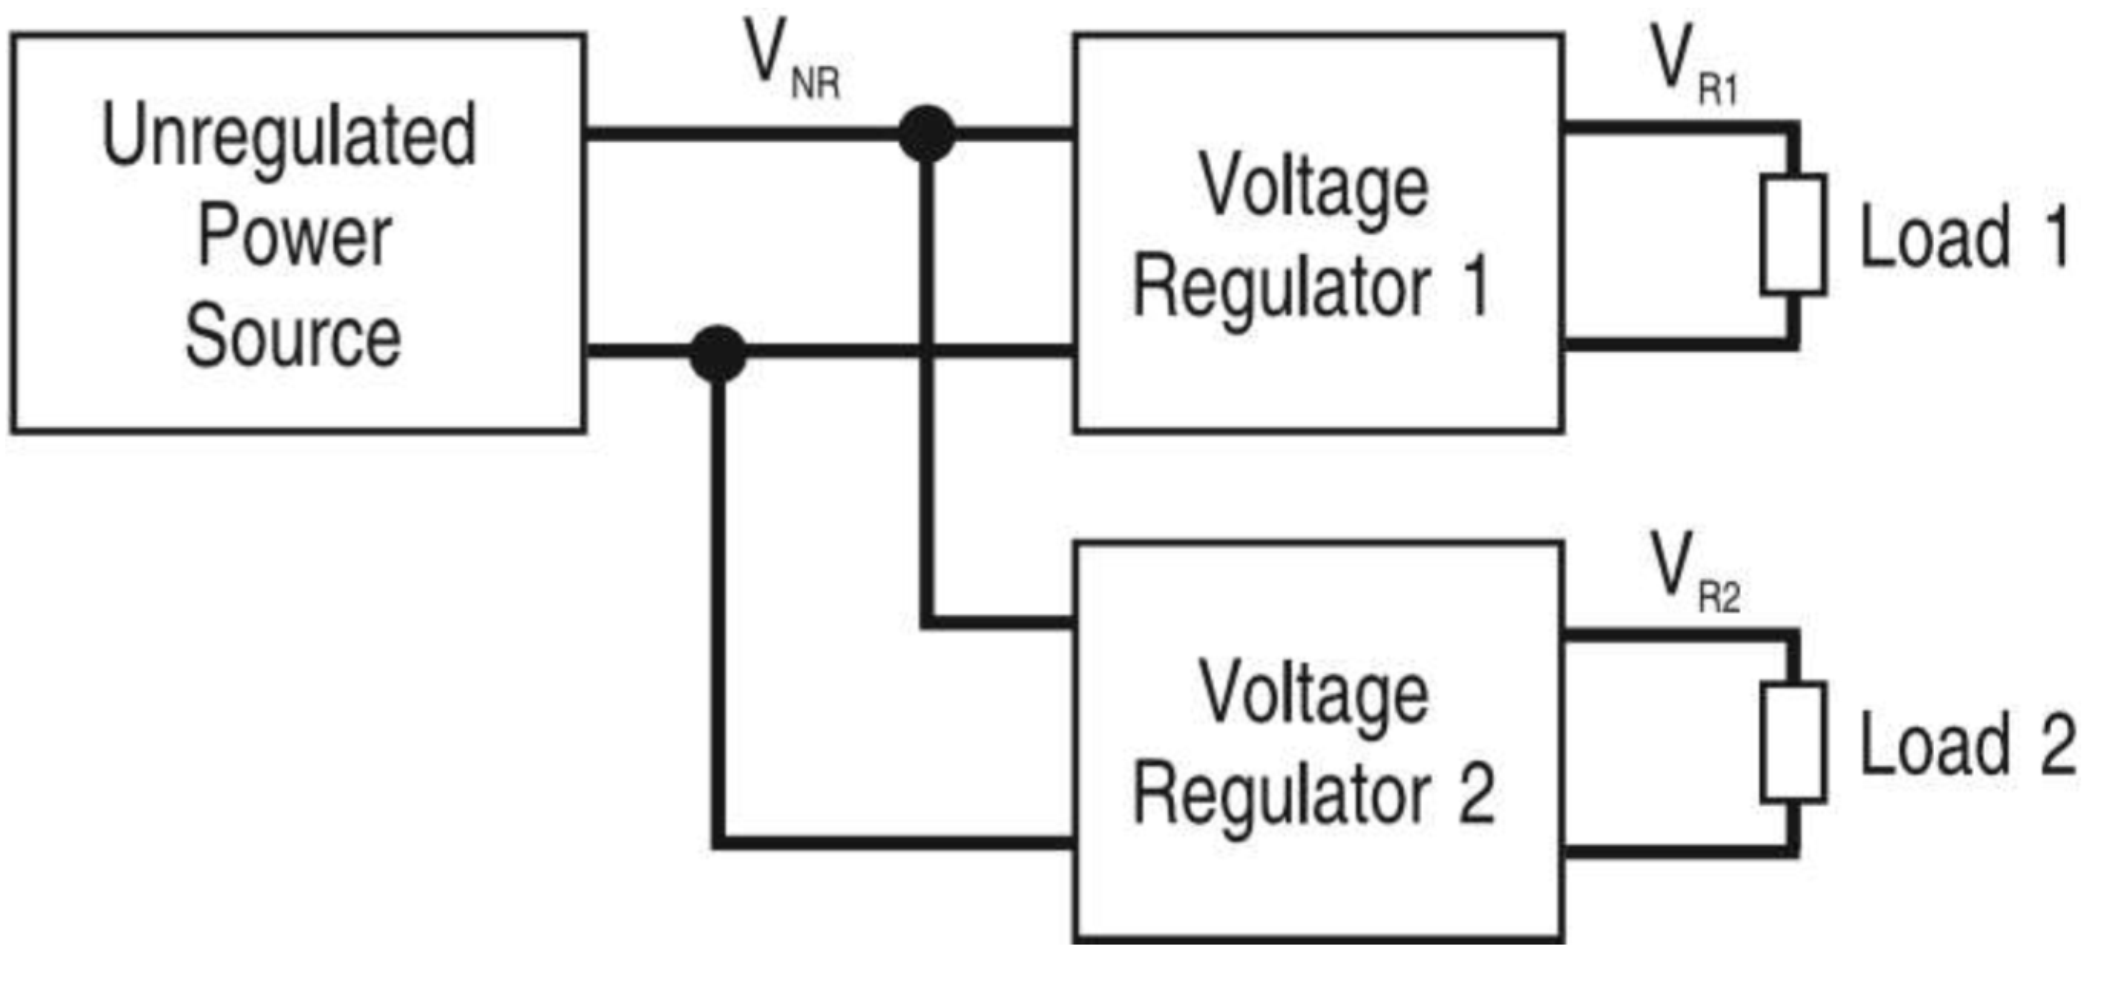
\includegraphics[width=7cm]{images/PowerSource.png}
\end{minipage}

\subsubsection{Terms of Power Sources \embsys{252}{?}}
\begin{minipage}{13cm}
	\begin{itemize}
		\item Power-Speed Tradeoff, link between frequency and power transfer
		\item Choose IC's with same Voltage as MCU
		\item For different IC Voltage Level, fix with Pull Up/Down Resistor
		\item For Noise Control use Capacitor between V and GND
        \subitem  $ \rightarrow $ act as a low-pass filter
		\item Isolate Power Sourcees from the Rest of the Circuit
		\item Route separately analog and digital lines 
		\item Do not mix analog and digital parts
	\end{itemize}
\end{minipage}
\begin{minipage}{5cm}
    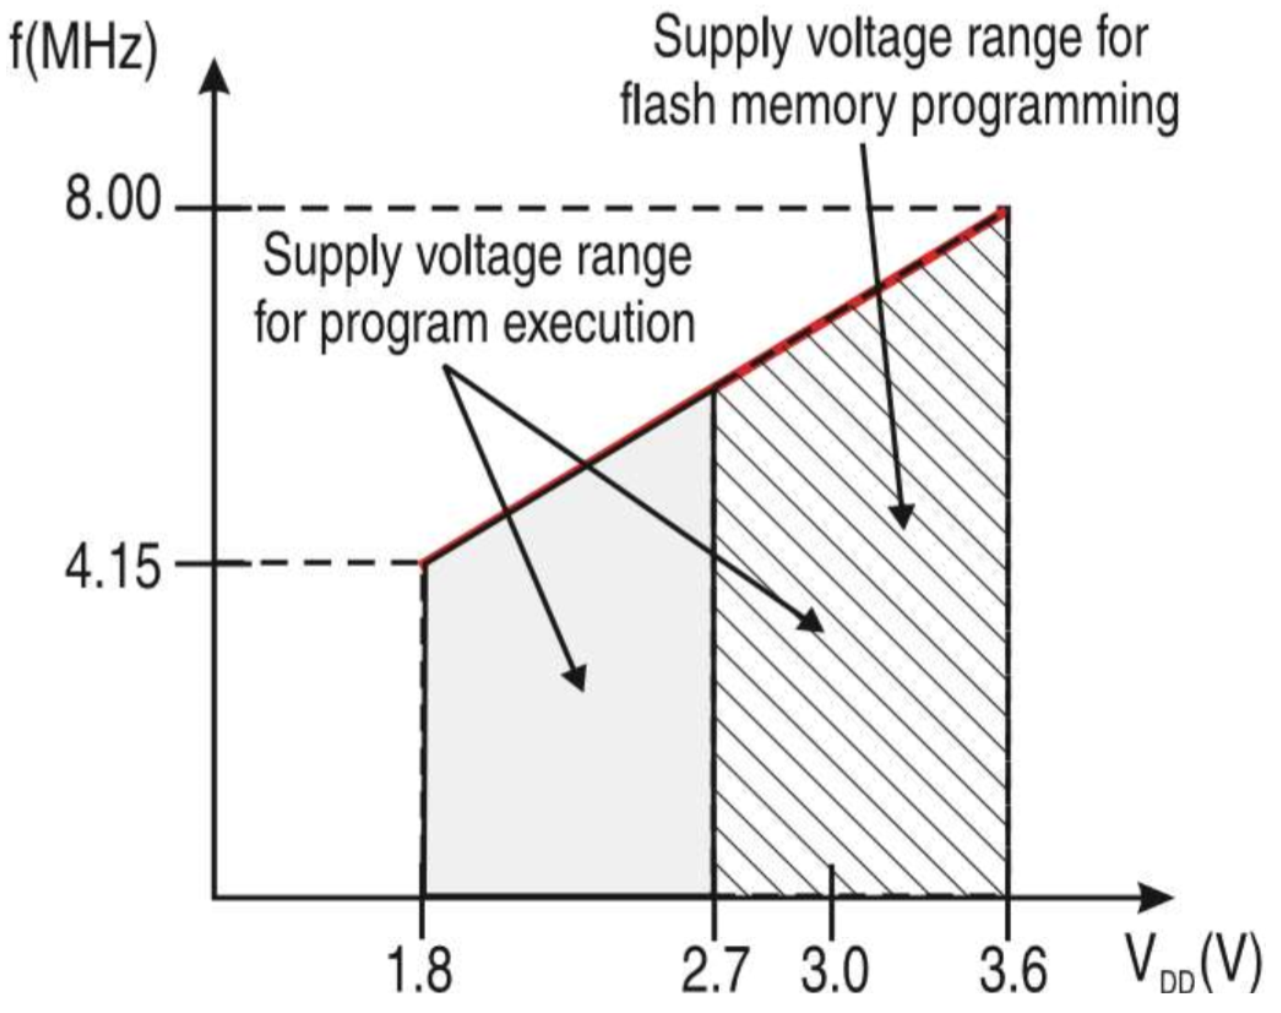
\includegraphics[width=6cm]{images/PSTradeoff.png}
\end{minipage}

\begin{tabular}{l l}
    \textbf{Regulator Capacity ($I_R$)}     & \textbf{Input voltage($V_{NR}$)} \\
    $ I_R \geq I_L = \sum_{i=1}^{n}I_{Li} $ & $ V_{NR} \geq  (V_R + V_D)$\\
    \textbf{Non-regulated capacity}         & \textbf{Non-regulated Power} \\
    $ I_{NR} \geq (I_R + I_{gnd}) $         & $ P_{NR}=V_R(I_R + I_{gnd}) $ \\
    \textbf{Power to load}                  & \textbf{Power Efficiency} \\
    $ P_R = V_R \cdot I_L $                 & $ Eff = \dfrac{P_R}{P_{NR}\cdot 100\%} $\\   
\end{tabular}
\begin{minipage}{2cm}
    {\scriptsize
    $V_R$ = regulated Volatge\newline
    $ V_D$ = dropout Voltage \newline  } 
\end{minipage}
\begin{minipage}{5cm}
    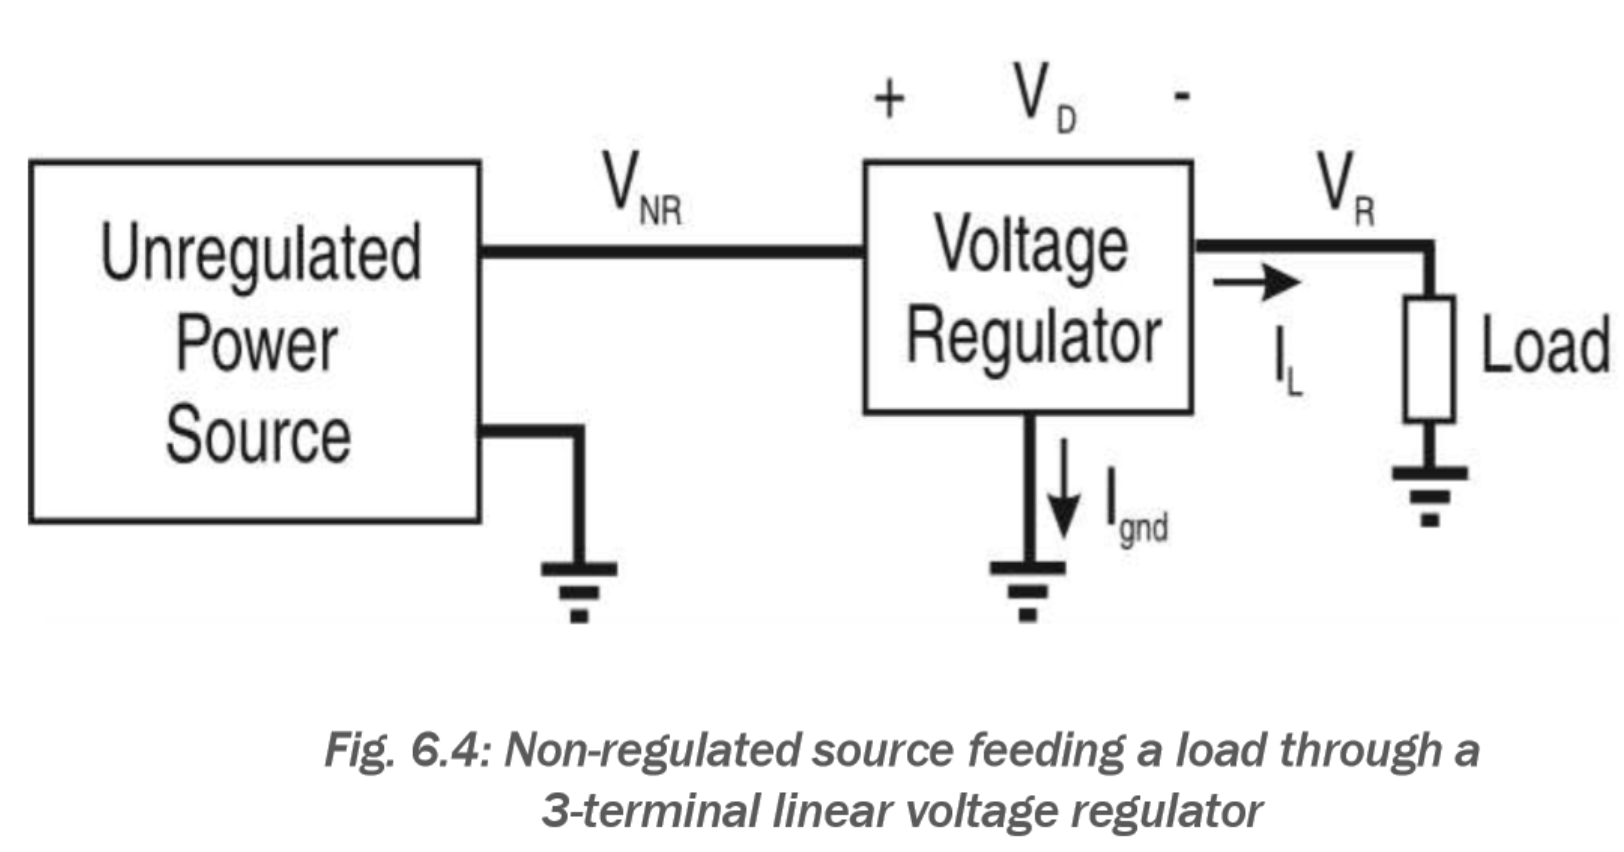
\includegraphics[width=8cm]{images/NRPowerSource.png}
\end{minipage}

\clearpage

\subsection{Clock Sources \embsys{260}{6.3}}
Clocks are usually based on quartz cristal oscillator. This oscillator is based on mechanical vibration using the piezoelectric effect. 
\begin{itemize}
	\item Embedded Systems need a steady clock
	\item Synchronous nature of CPU and peripherals
	\item Time Base for bus activity, timers, baud rates etc
\end{itemize}
\subsubsection{Parameters for Clock Signal \embsys{261}{6.3.1}}
\begin{minipage}{\linewidth}
    \centering
    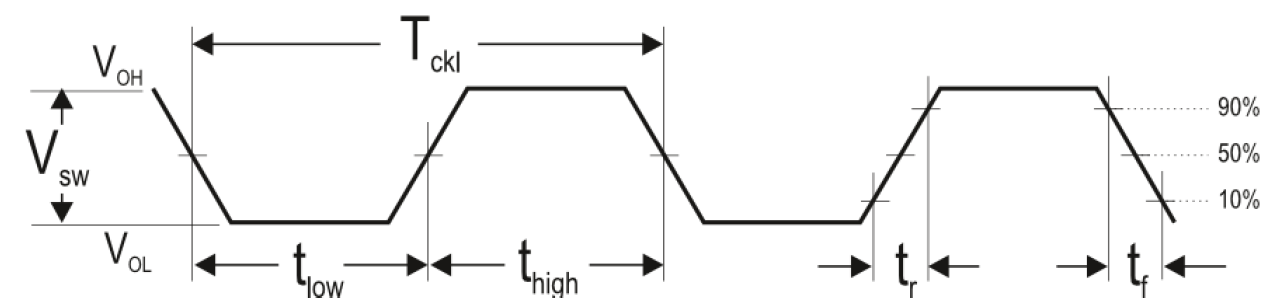
\includegraphics[width=0.7\linewidth]{images/clock_parameters.png}
\end{minipage}
\begin{minipage}{\linewidth}
    \begin{multicols}{2}
	\begin{itemize}
		\item \textbf{Voltage Swing} (Amplitude between low-high) $V_{SW}=V_{OH}-V_{OL}$
		\item \textbf{Frequnecy} (Number of Cycles per second) \\$f_{clk}=1/T_{clk}$
		\item \textbf{Duty Cycle} (Ratio of high time to period)\\ $DC=t_{high}/T_{clk} \cdot 100 \%$
		\item \textbf{Edge Speed} (Rising and falling times)\\$t_r, t_f$
	\end{itemize}
\end{multicols}
\end{minipage}

\subsubsection{Clock Stability \embsys{262}{}}
\begin{tabular}{ll}
	Clock Stability & Fluctuations of a clock signal over time intervall\\
	Clock Jitter & Randomness of signal passing voltage threshold\\
    Clock Drift & Change of frequency of an oscillator over time\\
\end{tabular}

\subsubsection{Choosing a ClockSource \embsys{264}{6.3.2}}
\begin{center}
    \begin{minipage}{7cm}
        \centering
        \textbf{Choose the frequency as low as possible, but as high as necessary}
    \end{minipage}
\end{center}

What is the fastets event the system will need to handle?\\
Has the value of $ V_DD $ been assigned?\\
What peripherals will share the same clockfrequency?\\
How precise does the clock need to be?\\
What are the capabilities of the Clock System in my MCU?

\subsubsection{Internal vs External Clock Source \embsys{265}{6.3.3}}
\begin{multicols}{2}
    \begin{minipage}{\linewidth}
        \textbf{Internal Clock}\newline
        RC, mostly used in MCU's
        \begin{itemize}
            \item [+] low number of Boardlevels
            \item [+] reducing area
            \item [+] reducing costs
            \item [+] low power consumption
            \item [-] Reduced clock stability
            \item [-] Less flexibility
            \item [-] Narrower bandwidth
        \end{itemize}
    \end{minipage}

    \begin{minipage}{\linewidth}
    \textbf{External Clock}\newline
    External Digital Clocks, RC or Quarz
    \begin{itemize}
        \item [+] more flexible
        \item [+] wider range of frequencies
        \item [+] larger drivin capabilities
        \item [+] high level of accuracy
        \item [-] increased number of Boardlevels
        \item [-] increased space
        \item [-] higher costs
    \end{itemize}
\end{minipage}
\end{multicols}

\subsubsection{RC Oscillators}
\vspace{-1cm}
\begin{minipage}{0.5\linewidth}
\begin{itemize}
    \item Based on PC phase shift circuit
    \item Clock stability depends on component tolerance
        \subitem R depends on temperatur
        \subitem D can $ V_DD $
    \item Limited bandwith   
\end{itemize}
\[ R_b = \dfrac{R_f}{2} \]
\[ \tau=R\cdot C \]
\[ f = \dfrac{1}{2 \pi RC} \]
\end{minipage}
\begin{minipage}{0.5\linewidth}
    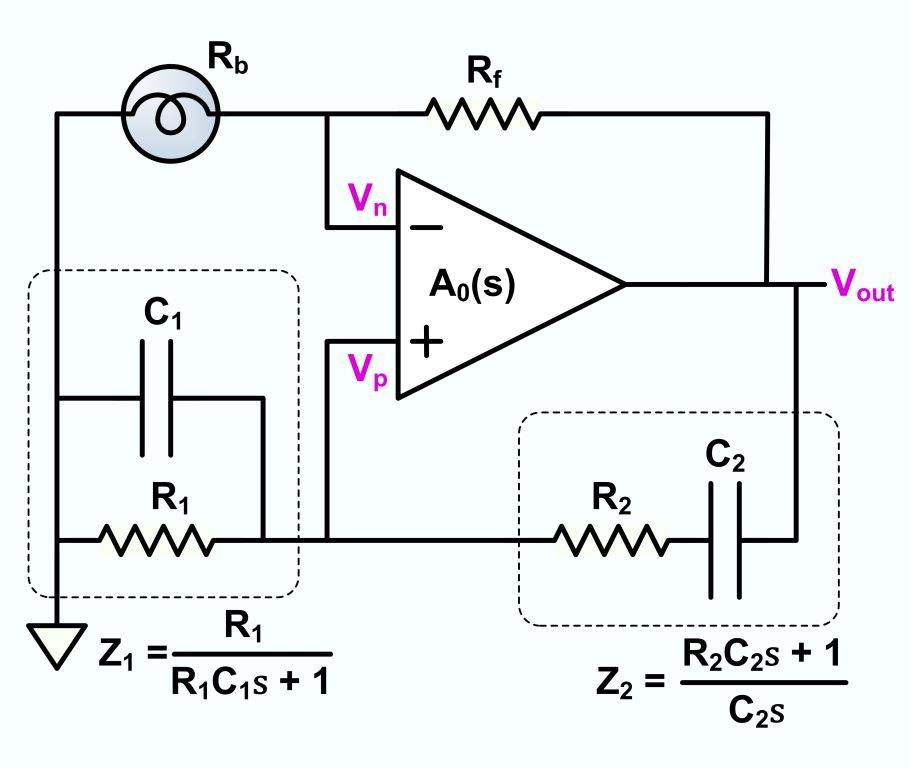
\includegraphics[width=\linewidth]{images/RCOscillator} 
\end{minipage}

\subsubsection{Quartz Crystal Oscillators \embsys{266}{6.3.4}}
\begin{minipage}{0.5\linewidth}
    \[ f_s=\dfrac{1}{2\pi \sqrt{L_1 \cdot C_1}} \]
    \[ f_p=\dfrac{1}{2\pi \sqrt{L_1 \dfrac{C_0 \cdot C_1}{C_0 + C_1}}} \]
\end{minipage}
\begin{minipage}{0.5\linewidth}
    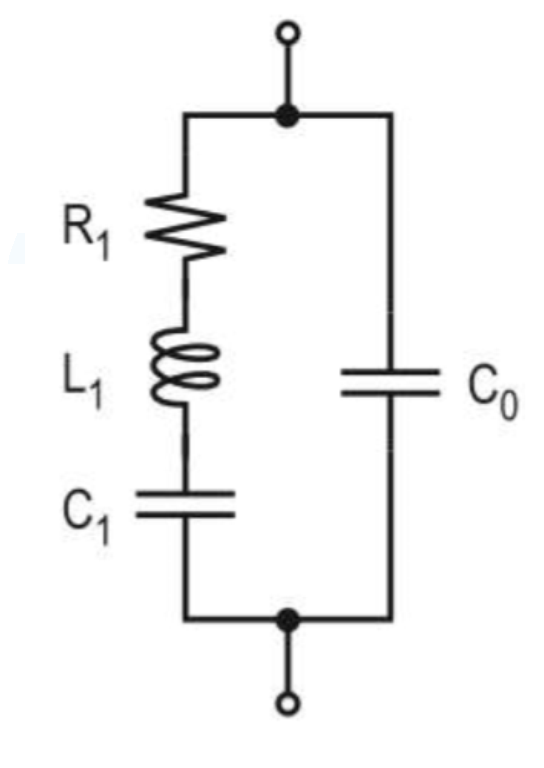
\includegraphics[width=0.3\linewidth]{images/QuartzESB} 
\end{minipage}
\begin{multicols}{2}
    \begin{minipage}{\linewidth}
        \textbf{Pierce Crystal Oscillator}\newline
        Series Resonant
        \begin{itemize}
            \item [+] low sensitivity to stray capacitors
            \item [+] low noise sensitivity
            \item [+] fast startup
            \item [-] High power consumption
            \item [-] can overdrive
        \end{itemize}
    \end{minipage}
    
    \begin{minipage}{\linewidth}
        \textbf{Colpitts Crystal Oscillator}\newline
       Parallel Resonant
        \begin{itemize}
            \item [+] low RF emission
            \item [+] low powerconsumption
            \item [+] 
            \item [-] Susceptial to noise
            \item [-] accelerated crystal aging
        \end{itemize}
    \end{minipage}
\end{multicols}

\textbf{Oscillator Startup Time \embsys{269}{}}\newline
What Causes the Startup Delay?\newline
%MAybe write some more stuff

\clearpage
\pagebreak